%\documentclass[%
%aip,
%jmp,
%amsmath,amssymb,
%reprint,%
%]{revtex4-1}
\documentclass{article}
\usepackage[margin=1.65in]{geometry}

\usepackage{graphicx}
\usepackage{dcolumn}
\usepackage{bm}
\usepackage[utf8]{inputenc}
\usepackage{amsmath}
\usepackage[english]{babel}
\usepackage{graphicx}
\usepackage[colorinlistoftodos]{todonotes}
\usepackage{tikz-3dplot}
\usepackage{adjustbox}
\usepackage{amsfonts}
\usepackage{pgfplots}
\usepackage{url}
\usepackage{algpseudocode}
\usepackage{algorithm}
\usepackage{siunitx}
\usepackage{subfig}
\usepackage[parfill]{parskip}
\usepackage{soul}
\usepackage{comment}


\addto\captionsenglish{\renewcommand{\refname}{Sources}}
\captionsetup{belowskip=0pt,aboveskip=4pt}
\pgfplotsset{compat=1.10}
\DeclareMathOperator{\sech}{sech}

\renewcommand\thesection{\arabic{section}}
\renewcommand\thesubsection{\arabic{section}.\arabic{subsection}}
\renewcommand\thesubsubsection{\arabic{section}.\arabic{subsection}.\arabic{subsubsection}}

\makeatletter
\def\p@subsection{}
\def\p@subsubsection{}
\makeatother

\newcommand\Tstrut{\rule{0pt}{2.6ex}}
\newcommand\Bstrut{\rule[-0.9ex]{0pt}{0pt}}
\newcommand{\TBstrut}{\Tstrut\Bstrut}

\newcommand{\comma}{\hspace{0.1mm},\hspace{0.7mm}}

%\setcounter{secnumdepth}{4}
%\setcounter{tocdepth}{4}

\pagestyle{empty}
\pagenumbering{gobble}

%Javascript LaTeX%
\usepackage{listings}
\usepackage{color}
\definecolor{lightgray}{rgb}{.9,.9,.9}
\definecolor{middlegray}{rgb}{.55,.55,.55}
\definecolor{darkgray}{rgb}{.4,.4,.4}
\definecolor{purple}{rgb}{0.65, 0.12, 0.82}
\definecolor{darkred}{rgb}{0.5, 0, 0}

\lstdefinelanguage{JavaScript}{
	keywords={typeof, new, true, false, catch, function, return, null, catch, switch, var, if, in, while, do, else, case, break},
	keywordstyle=\color{blue}\bfseries,
	ndkeywords={class, export, boolean, throw, implements, import, this},
	ndkeywordstyle=\color{darkgray}\bfseries,
	identifierstyle=\color{black},
	sensitive=false,
	comment=[l]{//},
	morecomment=[s]{/*}{*/},
	commentstyle=\color{middlegray}\ttfamily,
	stringstyle=\color{red}\ttfamily,
	morestring=[b]',
	morestring=[b]",
}

\lstdefinelanguage{HTTP}{
	keywords={GET, POST, null},
	keywordstyle=\color{blue}\bfseries,
	ndkeywords={query, form},
	ndkeywordstyle=\color{darkgray}\bfseries,
	identifierstyle=\color{black},
	sensitive=false,
	comment=[l]{\%},
	morecomment=[s]{/*}{*/},
	commentstyle=\color{purple}\ttfamily,
	stringstyle=\color{red}\ttfamily,
	morestring=[b]',
	morestring=[b]"
}

\colorlet{punct}{red!60!black}
\definecolor{background}{HTML}{EEEEEE}
\definecolor{delim}{RGB}{20,105,176}
\colorlet{numb}{magenta!60!black}

\lstdefinelanguage{JSON}{
	basicstyle=\normalfont\ttfamily,
	numbers=left,
	numberstyle=\scriptsize,
	stepnumber=1,
	numbersep=8pt,
	showstringspaces=false,
	breaklines=true,
	frame=lines,
	backgroundcolor=\color{background},
	morestring=[b]",
	stringstyle=\color{black}\ttfamily,
	literate=
	*{0}{{{\color{numb}0}}}{1}
	{1}{{{\color{numb}1}}}{1}
	{2}{{{\color{numb}2}}}{1}
	{3}{{{\color{numb}3}}}{1}
	{4}{{{\color{numb}4}}}{1}
	{5}{{{\color{numb}5}}}{1}
	{6}{{{\color{numb}6}}}{1}
	{7}{{{\color{numb}7}}}{1}
	{8}{{{\color{numb}8}}}{1}
	{9}{{{\color{numb}9}}}{1}
	{:}{{{\color{punct}{:}}}}{1}
	{,}{{{\color{punct}{,}}}}{1}
	{\{}{{{\color{delim}{\{}}}}{1}
	{\}}{{{\color{delim}{\}}}}}{1}
	{[}{{{\color{delim}{[}}}}{1}
	{]}{{{\color{delim}{]}}}}{1}
	{å}{{\r{a}}}{1}
	{ä}{{\"a}}{1}
	{ö}{{\"o}}{1}
	{Å}{{\r{A}}}{1}
	{Ä}{{\"A}}{1}
	{Ö}{{\"O}}{1}
	{...}{{{\color{darkgray}{...}}}}{1}
}

%\lstdefinestyle{numbers}
%{numbers=left, stepnumber=1, numberstyle=\tiny, numbersep=10pt}
\lstdefinestyle{nonumbers}
{numbers=none}

%\usepackage{lstautogobble}

\lstset{
	language=JavaScript,
	backgroundcolor=\color{lightgray},
	extendedchars=true,
	basicstyle=\footnotesize\ttfamily,
	showstringspaces=false,
	showspaces=false,
	%numbers=none,
	numbers=left,
	numberstyle=\footnotesize,
	numbersep=9pt,
	tabsize=2,
	breaklines=true,
	showtabs=false,
	captionpos=b,
	%autogobble=true
}

\lstset{literate=%
	{å}{{\r{a}}}1
	{ä}{{\"a}}1
	{ö}{{\"o}}1
	{Å}{{\r{A}}}1
	{Ä}{{\"A}}1
	{Ö}{{\"O}}1
}
%End Javascript%

\usepackage{xparse}

\NewDocumentCommand{\selector}{v}{%
	\texttt{\textcolor{darkred}{\textdollar}\textcolor{darkgray}{(}#1\textcolor{darkgray}{)}}%
}
\NewDocumentCommand{\regex}{v}{%
	\texttt{\textcolor{darkgray}{/}#1\textcolor{darkgray}{/}}%
}
%\newcommand{\selector}[1]{\verb|$(#1)|}}

\usepackage[numbers]{natbib}
\renewcommand{\bibfont}{\small}

\usepackage[titletoc,title]{appendix}

\begin{document}
	%\title[The process of retrieving schedule data from the Novasoftware web application]{The process of retrieving schedule data from the Novasoftware web application}
	\title{The process of retrieving schedule data from the Novasoftware web application}
	
	\author{John Rapp Farnes}
	%\affiliation{Värmdö Gymnasium}
	
	\date{\today}
	
	\maketitle
	
	\begin{abstract}\noindent
		The process of retrieving and extracting schedule data from the Novasoftware web application is derived and described, providing general instructions independent of programming language and platform. %The required theory is described, build on reliable sources. %Ska jag ta med det här?
		An implementation of the process is included, together with installation and usage instructions. Some possible applications are discussed and reviewed.
	\end{abstract}
	
	\newpage
	
	\tableofcontents
	
	\cleardoublepage
	\pagestyle{plain}
	\pagenumbering{arabic}
	
	\section{Introduction and background}
	I have observed that many Swedish schools including Värmdö Gymnasium, the high school that I attend, rely on the Novasoftware schedule application. I have further recognized that there is a general consensus among students that the web based schedule viewer provided with it does not reach the expectations of a modern application, especially considering its design and mobile experience. Because of this it may be of interest to create another viewing application, satisfying the needs of a modern application, using the schedule data provided by Novasoftware. Beacause Novasoftware provides no public API (Application Programming Interface) or other simple ways of extracting this data, a method of obtaining the information from the provided public interfaces is required.
	
	In the case of the high school I attend; the school provides a separate schedule for Tuesdays via an independent application. This inconvenience of using separate applications for different days further increases the relevance of extracting the Novasoftware data, in order to unify the two schedules into one. Also, when thinking about the implications of having access to this data I realized that it could be used for research purposes; analyzing the schedules of different schools and drawing conclusions from them.
	
	Any applications are outside the scope of this paper but are mentioned in order to interest the reader and because of their role as motivation for the project.
	
	\subsection{Purpose}
	%Lite mycket implement här
	The purpose of this paper is provide a complete documentation, as well as a working implementation, of the process of fetching, parsing and extracting data from the Novasoftware public web interface. 
	
	The purpose of the documentation is to act as a guide for implementation of the entirety or parts of the process. An implementation is included, providing a working program capable of extracting current schedule data. This data may for example be used to create custom viewers or for analysis. The documentations also acts as a description of the provided implementation so that it may be examined and reviewed.
	
	\subsection{Goals}
	The goal of this paper is to provide a documentation of the schedule extraction process that may be implemented in any programming language or platform, as well as including a working implementation, complete with installation and usage instructions.
	
	Further, the data derived from the presented process must be general and follow a logical format.
	
	The process should be if not in its original form, then with minor adjustments, applicable to every schedule provided by the Novasoftware application. Notes must be included where such adjustment may be neccecary.
	
	\subsection{Delimitaions}
	Because the Novasoftware schedule data and its formats appears to be at least in part manually input by school representatives with possibly varying conventions, it may not be consistent between schools or classes. Since not every case can be covered, the process described will be adapted to and only guaranteed to work on the current schedules from Värmdö Gymnasium. Despite this; tests on other schedules indicate that the process is applicable to most schedules with none or minor adjustments.
	
	The process has been developed for the current version of the Novasoftware application, as of the date of publication of this paper, and may not cover future versions.
	
	For obvious reasons only one implementation is included. The selected language is JavaScript, written for the Node.js platform. The reason behind this decision is convenience; that I feel comfortable with it. JavaScript is also suitable because of its close connection to the web.
	
	\subsection{Theory}
	
	The Novasoftware application is typically accessed via a web browser. A web browser (or simply browser) is a program capable of retrieving and displaying web content. The content is provided by a web server, usually as HTML (Hyper Text Markup Language) to the client (in this case the browser) via HTTP (HyperText Transfer Protocol) over the Internet.\cite{wikipedia web browser} A resource provided by a web server may be called an endpoint. In order to automate the process of fetching resources a different HTTP client than a browser is required. In the implementation Node.js is used to perform the requests. Node.js may be described in short as an environment for running JavaScript outside of the browser.\cite{wikipedia node.js}
	
	\subsubsection{HTTP-requests}
	An HTTP request is a message sent over the Internet from the client to a server. The server should then return a response containing the requested resource back to the client. HTTP requests are constructed of a URL (Uniform Resource Locator), a method, a set of headers and a request body.
	
	The URL acts as an address for the requested resource, comparable to how postal addresses are used for mail. A URL and consists of a protocol, a domain, a path and a query string. An example URL is\\
	\url{http://www.novasoftware.se/ImgGen/schedulegenerator.aspx?format=png}
	
	Here, the protocol is \url{http}, the domain is \url{www.novasoftware.se}, the path is \url{/ImgGen/schedulegenerator.aspx} and finally the query string is \url{?format=png}.
	The protocol denotes the type of request. In this paper only \texttt{http} and its secure counterpart \texttt{https} will be used. The domain specifies the server, while the path points to requested the resource on it. The query string is optional and may contain extra information about the request in a key-value structure. In the example above; the query string tells the server that the \texttt{format} should be \texttt{png}.
	
	HTTP requests also include a \texttt{method}, where only GET and POST will be used in this paper. The different methods differ in multiple ways. Foremost they include a notion of convention; where GET means that some information is to be fetched and POST means that some data is to be passed to the web server. A POST request may also include data to be passed to the server known as form data because of the traditional application of using forms to send it. In GET requests further information may instead be included in the URL query string, as specified above.
	
	An HTTP request further includes a set of headers, which provide more information about the request, again in a dictionary (key-value) structure. Headers may be divided into request - and response headers. Request headers sent from the client to the web server, while response headers are sent back to the client in the server response. The request headers may for example provide the server with information about the client, such as the software performing the request, while a response header can indicate for example if the requested action was successful or not. This is often indicated in the \texttt{Status} field. Another relevant header field is the \texttt{Location} response header. If it is provided, along with a 30X (300, 301 etc.) response status, the server is indicating that the resource is instead to be found at the URL provided in value of the \texttt{Location} header.\cite{wikipedia http request}\cite{wikipedia url}
	
	Another important feature of HTTP requests are that they can include cookies. Cookies are used by applications in order to save small amounts of data in the browser and are sent back and forth in every request. This is often used to give the client an ID (Identifier) so that information about the client can persist between sessions even though HTTP is a stateless protocol.\cite{wikipedia cookie}
	
	\subsubsection{HTML}
	Because the HTML obtained from the server response is a string, there is a need to transform it into a searchable and more practical structure. Often the document is described in a DOM (Document Object Model), providing a more programmer friendly interface. In order to reference certain locations or data points of the HTML documents, CSS (Cascading Style Sheets) selectors are used, because of their popularity within the web. The method used in this process, where HTML is retrieved and information is extracted from it in an automated program, is often referred to as web scraping.\cite{wikipedia css}\cite{wikipedia web scraping}
	
	\subsubsection{JSON}
	The output of the program is in the JSON (JavaScript Object Notation) format which is human readable and particularly useful for the web because of it's similarity to JavasScript; the de facto scripting language on the web.\cite{wikipedia json}
	
	\subsubsection{PNG and PDF}
	In the process, the PNG (Portable Network Graphics) and PDF (Portable Document Format) file formats are encountered. PNG is an image format, while a PDF is a document format. The relevant information about PDF documents are that they consist of pages, texts and fills (indicating parts of the document filled with color).\cite{wikipedia png}\cite{wikipedia pdf}
	
	\subsubsection{Regular expressions}
	Regular expressions are used in multiple instances in the parsing process. A regular expression is a pattern designed to match (indicating if a string belongs to) a particular set of strings. The set is described using symbols, indicating different characters or operators.\cite{wikipedia regex}
	
	\subsection{Conventions}
	Examples will be written in JavaScript. An ES5 (ECMAScript 5) or later environment is assumed. JavaScript code is syntax highlighted and look as such:
	\begin{lstlisting}[language=JavaScript]
	var string = 'Hello world!'; //This is a comment
	console.log(string);
	\end{lstlisting}
	
	Variables, object fields, keywords etc. are displayed in a \texttt{monospace font}.
	
	URLs look like the following:\\
	\url{http://www.example.com/path?author={name}}\\
	The brackets denote variable substitution. In the above expression, the value of the variable \texttt{name} is to be substituted after the slash. If for example the value of the \texttt{name} variable is the string "john", the resulting URL would be:\\
	\url{http://www.example.com/path?author=john}
	
	HTTP request are displayed as such:
	
	\newpage
	\begin{lstlisting}[language=HTTP, style=nonumbers]
	POST
	http://www.example.com/publish
	query: {
		type: {type}
		reason: school project
	}
	form: {
		author: {author}
		experience: null
	}
	\end{lstlisting}
	The first row indicates the HTTP method, while the second denotes the URL. The \texttt{query} dictionary describes the key-value entries of the query string to be included in the URL. The form \texttt{form} field exists only on POST requests and specifies the request form data. A \texttt{null} value denotes an empty value.\\
	The above description, with the variable \texttt{type} set to "paper" and \texttt{author} set to "john", should result in a POST request to the URL \url{http://www.example.com/publish?type=paper&reason=school%20project}%Textstudio bug
	, with form data fields equivalent to \texttt{experience=\&author=john}.
	
	%Kanske inte borde vara färg på selectors, men det är nice om de sticker ut lite
	CSS selectors will be written \selector{selector}, for example \selector{div} would select all the \texttt{div}s in the document.
	
	Regular expressions will be written as such \regex{expression}, for example \regex{^\d} would match all strings starting with a digit. Regular expression features and behavior of ES5 or later is assumed.
	
	\subsection{Method}
	The process has been derived via a series of experiments and attempts. The data and different HTTP endpoints have been discovered while attempting to reverse engineer the application by navigating and examining the different pages. Ways of reaching these using a non-browser client has been determined via trial and error.
	
	The parsing method was derived by first studying different schedules; examining how they were organized and how the information could be extracted. From these schedules certain conclusions about the structure of the data could be drawn and using these an algorithm was proposed. Once implemented, this algorithm was tested on multiple schedules and tweaked until all (detected) errors were eliminated. In some cases a solution originally proposed was discovered to be insufficient and a new solution was sought.
	
	The HTTP requests used in the process were found by imitating the web browser's request when using the Novasoftware application. These requests were accessed and viewed using the browser development tools. Because the requests often include redundant information, such as empty header or form data fields, only the relevant information was kept in order to make the requests as simple and elegant as possible. These were determined by the process of experimentation and elimination.
	
	\subsection{The Novasoftware application}
	In order to explain and understand the process, knowledge of the Novasoftware application is required.
	
	The application consists of the following relevant endpoints:
	
	\subsubsection{The index page}
	The index page is the page first encountered by the user.
	
	\begin{figure}[h]
		\centering
		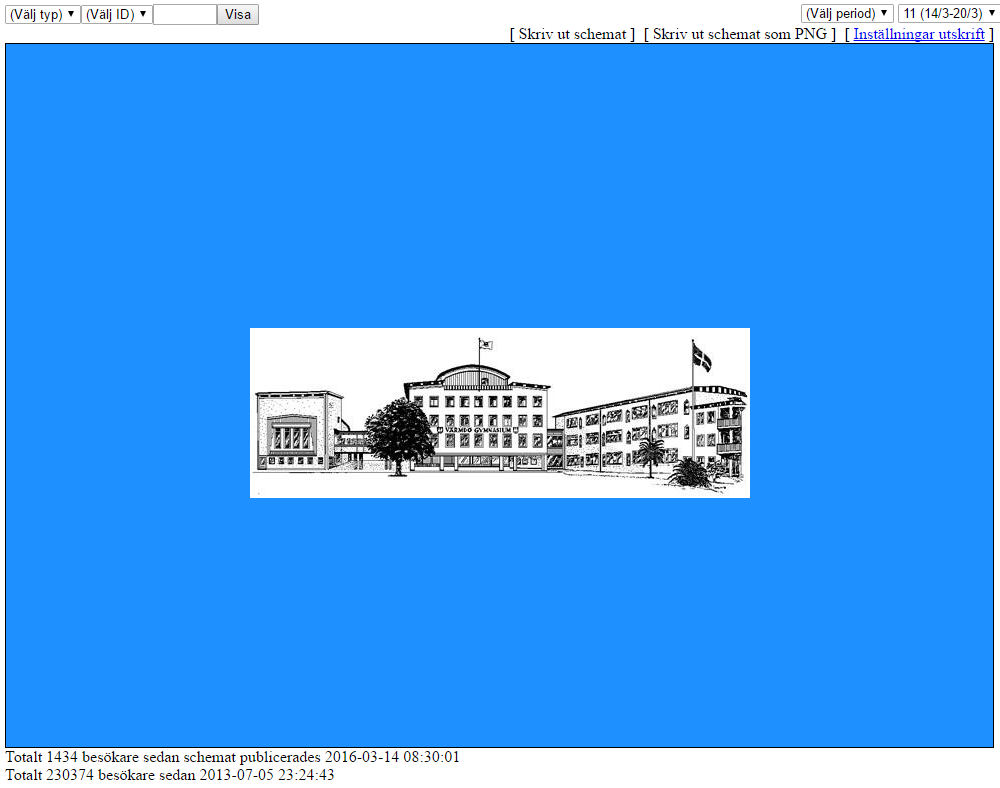
\includegraphics[width=0.9\linewidth]{images/index-page}
		\caption{}
		\label{fig:index-page}
	\end{figure}
	
	The page URL is
	
	\url{http://www.novasoftware.se/WebViewer/{novasoftware-id}/MZDesign1.aspx?schoolid={schoolId}&code={code}}
	
	The page is provided as HTML.\\
	In the selects in the top left section of the page, a class may be selected.\\
	In the selects in the top right section of the page, a week may be selected.
	
	Once a class is selected, the schedule page is presented.
	
	\newpage
	
	\subsubsection{The schedule page}
	
	The schedule page is the page that the user views in order to see their schedule.
	
	\begin{figure}[h]
		\centering
		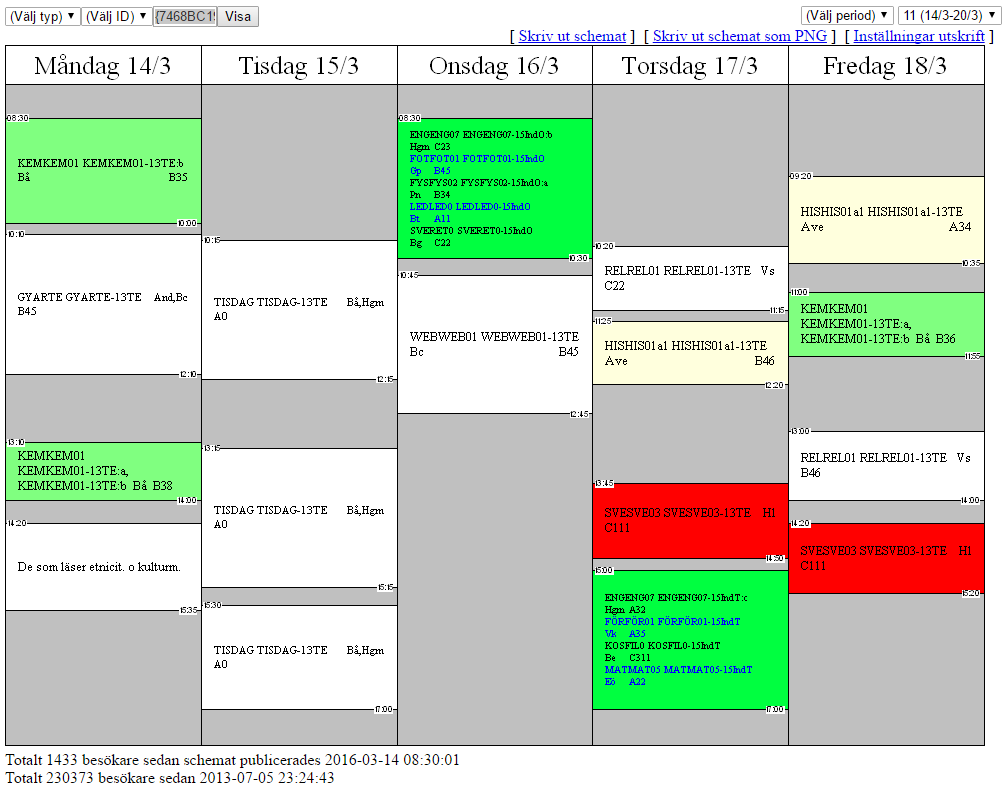
\includegraphics[width=0.9\linewidth]{images/schedule-page}
		\caption{}
		\label{fig:schedule-page}
	\end{figure}
	
	The page is provided as HTML, however the schedule is displayed as a PNG image.
	Via inspection using the browser development tools, the URL for this image can be obtained, which leads to the image endpoint.
	
	\subsubsection{The image endpoint}\label{image endpoint}
	The URL of the image endpoint is
	
	\url{http://www.novasoftware.se/ImgGen/schedulegenerator.aspx?schoolid={schoolid}&id={class-id}&format={format}}
	
	By default, the image endpoint returns a PNG of the selected schedule, however if the URL query string parameter \texttt{format} is changed from \texttt{png} to \texttt{pdf}, a PDF file is returned instead.
	
	\begin{figure}[!h]
		\centering
		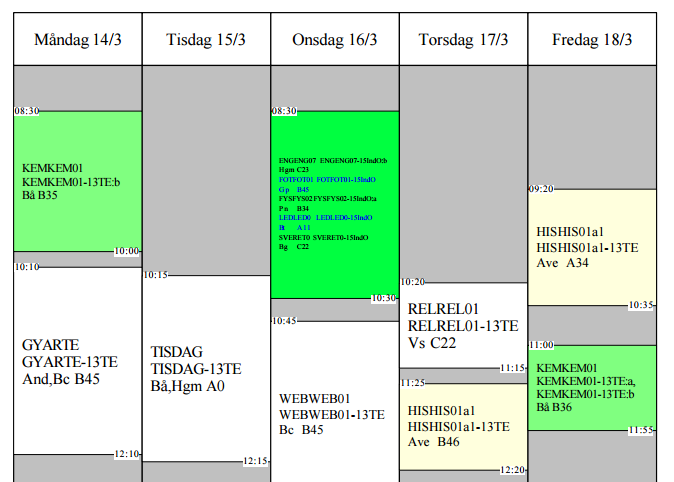
\includegraphics[width=0.6\linewidth]{images/schedule-pdf-cropped}
		\caption{}
		\label{fig:schedule-pdf}
	\end{figure}
	
	\subsubsection{The lesson detail page}
	Going back to the schedule page, a lesson can be clicked on. This redirects the browser to a detail page, providing additional information about the lesson in the HTML format.
	
	\begin{figure}[!h]
		\centering
		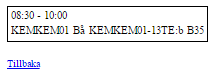
\includegraphics[width=0.5\linewidth]{images/lesson-page}
		\caption{}
		\label{fig:lesson-page}
	\end{figure}
	
	\section{Planning}
	%Vet inte om jag skulle kalla denna section planering. Förutom det första korta stycket diskuterade du mer om hur du ville att ditt API skulle se ute. Planning så tänker jag mer i vilken ordning saker ska göras och så.
	The planning phase of the project involved studying the Novasoftware web application and attempting to find endpoints that could be used. Because no public data API was found, it was determined that scraping was required.
	
	By observing the schedules; the data fields and structure were determined. The schema is included in  appendix \ref{schedule format}. Each schedule is associated with a \texttt{className}, a \texttt{week} and a list of \texttt{days} as well as a list of \texttt{lessons}.
	For each lesson there is a \texttt{startTime}, \texttt{endTime}, \texttt{day} and a \texttt{details} list.
	
	The details list items are composed of a \texttt{course}, \texttt{location} and a \texttt{teacher}. The details are in a list because it was observed that sometimes one lesson item on the schedule may include multiple lessons, as demonstrated below.
	
	\begin{figure}[h]
		\centering
		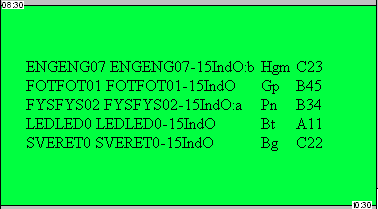
\includegraphics[width=0.5\linewidth]{images/multiple-lessons}
		\caption{}
		\label{fig:multiple-lessons}
	\end{figure}
	
	The \texttt{detail} list will contain only one entry in the most common case, where there is only one concurrent lesson. Otherwise it will contain one entry per lesson.
	
	\section{Development}
	
	\subsection{Viewing schedules using an HTTP client}
	Originally there were problems viewing the index page using a non browser HTTP client. The server responded with a redirect response instead of providing the HTML. Upon inspecting the URL it was noticed that it appeared to contain an ID which had previously been assumed to be a part of the path. An example of such an ID is highlighted in the URL below.
	
	\texttt{http://www.novasoftware.se/WebViewer/\hl{(S(310b0lvc2tbhmb451vdk4c2v))}\\/MZDesign1.aspx}
	
	Because the URL was originally copied from the browser, the ID was copied along with it and also used in the HTTP client. It was discovered that the URL ID varied between sessions when using the browser and the conclusion was made that the ID was invalidated after a certain amount of time. This lead to the problems with the HTTP client because an old and invalidated ID was used. To solve this, it proved useful to leave the ID out of the URL as such:
	
	\url{http://www.novasoftware.se/WebViewer//MZDesign1.aspx}
	
	The server would return a redirect response with a new URL containing a valid ID that could be used in future requests. However performing POST requests to this new URL, essential to the process, would produce a 500 (Server Error) response instead of the requested resource. By examining the browser activity and through the process of experimentation, it was discovered that if a GET request was first sent to the URL, subsequent POST requests would yield the appropriate response. It was as if the ID had to be "activated" before it could be used.
	
	\subsection{Parsing the schedule}
	Next a method of parsing the schedule was sought. The originally discovered representation of the schedule, a PNG-image, was impractical for parsing because images are notoriously hard to decode and extract information from. Instead a different format was desired, which lead to the vital discovery of the PDF version; a format much better suited for information extraction. Because the raw PDF format is hard to read, a parser was sought. JSON was determined to be a appropriate and a PDF to JSON parsing library was found. The next step was extracting the schedule information from this JSON result.
	
	\subsection{Extracting schedule information}
	The structure of the parsed result is included in appendix \ref{parsed pdf}.
	
	By studying the result the conclusion was made that the \texttt{Fills} corresponded to lessons and the \texttt{Texts} to lesson information as well as start and end times. The days of the lesson fills and texts could be determined by their x-coordinates. The problem was determining which lesson fill corresponded to which texts.
	\newpage
	\subsection{Associating lesson fills with lesson texts}
	The first approach proposed for reading the schedule was to do so in a linear fashion; one lesson at a time from top to bottom. The problem with this method was that multiple concurrent lessons was very common. This was especially prevalent in some particular schedules, such as the one below:
	
	\begin{figure}[h]%Lite röda ringar som visar där tider saknas
		\centering
		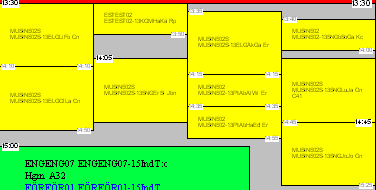
\includegraphics[width=0.7\linewidth]{images/schedule-13esmu}
		\caption{}
		\label{fig:schedule-13esmu}
	\end{figure}
	
	This problem was solved based on the observation that the texts corresponding to a fill always was contained by the correct fill, and no other. Because the fills and texts were described as rectangles (with a corner coordinate and a width and height), the texts for a particular fill could be found using a simple rectangle intersection test.
	
	\begin{figure}[!h]
		\centering
		
\includegraphics[width=0.1\linewidth]{images/rectangles-intersecting}
		\caption{}
		\label{fig:rectangles-intersecting}
	\end{figure}
	
	Another problem that had to be solved was that start or end times were not always assigned to lessons. Instead, if multiple lessons started at the same time, the time text was only placed on the leftmost lesson. This also applies to end times and can be seen in the above image. The initial solution for the problem was to search among the neighbors of the lessons missing times. However this solution proved unstable and could not successfully parse every schedule. Instead, when thinking about how we humans understand such a schedule, the fairly obvious but very useful observation was made that the times were always along the same horizontal line as the start or end bounds of the lessons. This is how us humans read the schedule; if there is a lesson that for example lacks a start time, we look along the same line until we find a lesson with a start time. Using this method, the missing times could be found by performing rectangle-line intersection tests.
	%Det här stycket är skrivet väldigt likt en blog post och skiljer sig ganska mycket från tidigare bitar av paperet. Det är inte nödvändigtvist fel och det beror på hur formellt man vill att slutresultatet ska vara. Jag har ingen CS erfarenhet men jag hade inte förväntat mig sånt här språk i ett MatFy paper.
	
	On some schedules, it was noticed that some times are not written out in full, but instead showing only the minute (as found in figure \ref{fig:pdf-no-text}). This was however easily solved by finding the closest above time and completing with its hour. In some cases, where the next hour has started, the hour has to be incremented by one.
	
	\subsection{Determining lesson details}
	The lesson texts had now been found and a way of extracting the lesson information from them described in the output format (such as the course) was needed. This was tricky because of inconsistencies between schedules and many edge cases were encountered in certain schedules. Some lessons for example lacked information about the location or would include extra fields, making it difficult to detect the relevant ones. A solution keeping as general as possible, but still capturing all the cases, was sought. Unfortunately methods of detecting a course, location and teacher were required, losing some generality because the definitions may differ between schedules. This was primarily done via the use of regular expressions.
	
	\subsection{Incomplete lessons}
	It was quickly discovered that a problem with the PDF verison of the schedule was that some lessons lacked text. This was especially prevalent where the lessons were very small and densely packed.
	
	\begin{figure}[h]
		\centering
		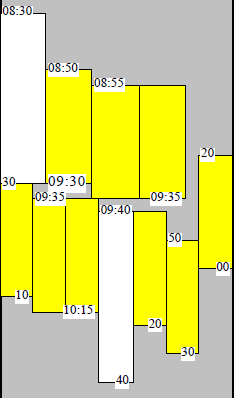
\includegraphics[width=0.3\linewidth]{images/pdf-no-text}
		\caption{}
		\label{fig:pdf-no-text}
	\end{figure}
	
	These lessons had to be completed from another source.
	
	\subsection{Completing lessons}
	As described in section \ref{image endpoint} when clicking within the bounds of a lesson on the schedule page, a detail page would load containing the information of that particular lesson. This was exploited in order to fetch information for the incomplete lessons without text since this was available for every lesson.
	
	It was discovered that the request that had to be performed in order to simulate the click contained the x and y coordinates for the click as well as the width and height of the schedule image that was being clicked upon. The next problem to determine these coordinates.
	
	\subsection{Determining the click coordinates}
	A set of coordinates were used in the PDF for the text and fills, but these did not match with the image. Below is a illustration of a image and PDF of the same width and height layered on top of each other. Note the mismatch.
	
	\begin{figure}[h]
		\centering
		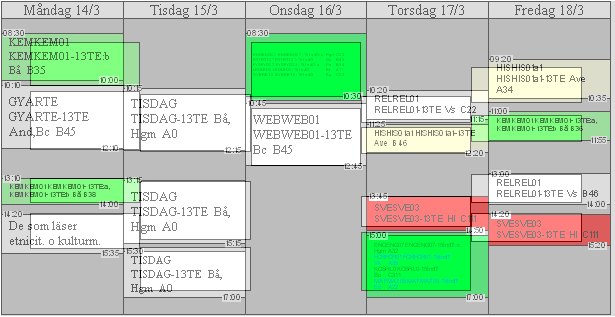
\includegraphics[width=0.7\linewidth]{images/pdf-image-mismatch}
		\caption{}
		\label{fig:pdf-image-mismatch}
	\end{figure}
	
	From the above figure one can see that the PDF lessons start further from the edges than the image. The misfit was assumed (which turned out to be correct) to be linear, meaning that the displacement was a linear function of the coordinates. This enabled the use of a simple linear transformation to correct for it, scaling and translating every x and y coordinate by a constant amount. If $P = (x, y)$ denotes the original position and $P' = (x', y')$ denotes the transformed and corrected result the equation for this process may be described in the following way.
	
	\begin{eqnarray}
		P' &=& (s_x*x + t_x, s_y*y + t_y)\nonumber\\
		\implies x' &=& s_x*x + t_x, \nonumber\\
		y' &=& s_y*y + t_y \nonumber
	\end{eqnarray}
	
	The width was also scaled with a constant $s_w$ because the ends did not match up perfectly.
	
	The constants for these transformations was found by the process of experimentation and are included in appendix \ref{constants}. With these constants an almost perfect match was achieved as displayed below.
	
	\begin{figure}[h]
		\centering
		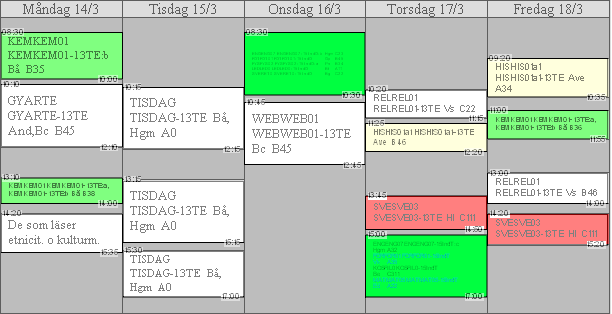
\includegraphics[width=0.7\linewidth]{images/pdf-image-match}
		\caption{}
		\label{fig:pdf-image-match}
	\end{figure}
	
	\textit{Please note that the included constants only work for PDFs displaying the schedule horizontally, as is the case for the majority of schedules I have encountered, including Värmdö Gymnasium but not for example the Stockholm high school Norra Real. Because the displacement in vertical schedules is also linear, the same method may be used using a new set of constants.}
	
	\subsection{Performing the click}
	When performing the click the center coordinates were determined to give the best accuracy; reducing the risk of missing because of calculation error. These were calculated by averaging the corner coordinates.
	
	The click simulation process works as follows: First a request is sent containing the coordinates. The server responds with a redirect request, pointing to the lesson detail page. The new URL obtained in this request is however static and does contain any information about which lesson was pressed. This was a problem when attempting to simulate the process with the HTTP client. After examination it was determined that this information was contained as an ID in the cookie, returned when requesting the schedule and was then expected to follow with the click request. This meant that a schedule first had to be fetched to get this cookie. In order to reduce the overhead of this request a PNG with dimensions 1 x 1 was requested.
	
	\subsection{Reading lesson information from HTML}
	The response of the final click request was the lesson detail page, provided as HTML. The relevant information was relatively easily found because they were contained in a table and could be obtained using standard HTML traversal methods.
	
	\subsection{Failing requests}
	It was noticed that some requests, in a seemingly random pattern, failed (produced no response). In order to continue the process the requests had to be retried and performed again. This applied especially to the click requests. After examining this problem, the cause seemed to be performing too many request too fast and with too little space in between. In order to solve this, all requests were made in sequence and a timeout was performed before making the next request. In order to determine which timeout time was optimal in order to minimize the total time to parse schedules (which is especially important when parsing many schedules) experiments were made. These experiments were performed by completing the process using a certain timeout and measuring the total time elapsed. If the timeout time was too short certain request failed and had to be retried, taking a lot of time. On the other hand, if it was too long, time was wasted. The resulting value was 100 milliseconds. Please note that the optimal time may be dependent on the system or Internet connection and may therefor not be appropriate for every setup.
	%Bra skriven sektion. Speciellt 3.5 framåt hade bra språk och det är ju intressant på riktigt att läsa om hur alla problemen hanterades.
	
	\section{Results}
	In this section the final process to fetch, parse and extract information from schedules is presented.
	
	In order to perform the requests an ID is required to specify the school from which the schedules is to be fetched for. The ID can be found as the \texttt{schoolid} in the query string of the URL when viewing the schedule as a regular user. From the query string, take the \texttt{code} also as it is required for some requests. For Värmdö Gymnasium the \texttt{schoolid} is \texttt{99810} and the \texttt{code} is \texttt{945537}.
	
	\subsection{Obtaining a Novasoftware ID}
	Next, a Novasoftware ID must be obtained. First perform the following request:
	
	\begin{lstlisting}[language=HTTP, style=nonumbers]
	GET
	http://www.novasoftware.se/WebViewer//MZDesign1.aspx
	query: {
		schoolid: {schoolId}
		code: {code}
	}
	\end{lstlisting}
	
	The response will contain a \texttt{Location} header. Save this in a variable \texttt{path} as it contains a URL with an ID. Second, in order to "activate" the page, perform the following request:
	
	\newpage
	\begin{lstlisting}[language=HTTP, style=nonumbers]
	GET
	http://www.novasoftware.se{path}
	query: {
		schoolid: {schoolId}
		code: {code}
	}
	\end{lstlisting}
	
	\subsection{Class IDs and weeks}
	In order to request a schedule, the \texttt{classId} must first be fetched, which may be found by performing the following request
	
	\begin{lstlisting}[language=HTTP, style=nonumbers]
	POST
	http://www.novasoftware.se{path}
	query: {
		schoolid: {schoolId}
		code: {code}
	}
	form: {
		__VIEWSTATE: null
		__EVENTTARGET: TypeDropDownList
		TypeDropDownList: 1
		ScheduleIDDropDownList: 0
		PeriodDropDownList: 8
		WeekDropDownList: {week}
	}
	\end{lstlisting}
	
	The server will respond with an HTML document. The list of IDs may be found with the following selector \selector{#ScheduleIDDropDownList option}. The class names are obtained as the text contents of the options elements and the IDs as their HTML \texttt{value} attributes.
	
	On this page, the available weeks can also be read as the values of the option elements returned by the selector \selector{#WeekDropDownList option}.
	
	\subsection{Fetching the schedule PDF}
	Now that a classId has been obtained, the schedule PDF may be reached with the following request:
	
	\begin{lstlisting}[language=HTTP, style=nonumbers]
	GET
	http://www.novasoftware.se/ImgGen/schedulegenerator.aspx
	query: {
		schoolid: {schoolId}
		id: {classId}
		week: {week}
		format: pdf
		period: null
		width: 1
		height: 1
	}
	\end{lstlisting}
	
	\subsection{Parsing the schedule PDF}
	The PDF has to be parsed into JSON or another equivalent structured format. In the parsed result, find the \texttt{Fills} and the \texttt{Texts} as well as the \texttt{Width} and \texttt{Height} as these are the relevant fields. The width must be scaled with the constant $s_w$. In the parsed result, the coordinates origin is in the top left corner, with x and y ascending to the right and down. Sort the texts by ascending y coordinate, with those sharing the same y coordinate sorted by ascending x coordinate.
	
	\subsubsection{Determining and preparing the lessons fills}
	Starting with the fills, we first want to select which fills belong to lessons. Assign a variable for the lesson fills and include all the fills that match the following conditions:
	\begin{description}
		\item[$\bullet$] Non empty, i.e width and height $>$ 0
		\item[$\bullet$] Not a title fill, width != 18.391 and height != 2.75
		\item[$\bullet$] Not too high, height $<$ 46
		\item[$\bullet$] Not too small, area (width x height) $>$ 2
	\end{description}
	
	Next the lesson fills must be transformed to match the image. Calculate the corrected x and y coordinates using the formulas $x' = s_x*x + t_x$ and $y' = s_y*y + t_y$. Next the center x and and y are determined by averaging the corner coordinates, while the day is determined by dividing the center x with the total width and multiplying by 5 (the amount of days in a school week). The result must be floored, i.e rounded down to the nearest integer. Now, 0 denotes Monday and 4 denotes Friday etc.
	
	\subsubsection{Separating the texts}
	It was discovered that the text positions does not perfectly match up with the lesson positions. To compensate for this, they must be offset slightly using the following formula $x' = x + t_{tx}$ and $y' = y + t_{ty}$ (see appendix \ref{constants}). Because the texts are too big to fit inside the lessons, set the width and height to $w_t$ and $h_t$. Next, in order to compare the text positions to the lessons, the above transformation must be applied to them also.
	
	The texts are divided in to three parts; lesson texts, time texts and title texts (which are used in the \texttt{days} field, see appendix \ref{schedule format}).
	
	Because of how the texts are sorted, the title texts will be the first five texts. Assign these to a variable and remove them from the texts array.
	
	Now, each remaining text is either a time or lesson text. They can be separated because time texts follow the same format HH:MM. Some times however are displayed only partial, showing only the minute as seen in figure \ref{fig:pdf-no-text} on page \pageref{fig:pdf-no-text}. For each text, the texts that match the expression \regex{^\d{2}:\d{2}$} %$ 
	are considered a time and the texts that match \regex{^\d{2}$} %$
	are considered partial times. The partial times may be completed by finding the closest above time text and taking its hour (the first two digits), appending the minute in the partial text to it. Since a new hour may have started between the partial time and the above time; increment the hour by one if the minute of the partial time is less than the minute of the above time. Now, the rest of the texts are considered lesson texts.
	
	\subsubsection{Finding the start and end times of lessons}
	Next the start and end time are sought for the lessons. For each fill; find all the time texts which bounding rectangle is intersected by the horizontal line of the lesson top bound using a line-rectangle intersection test. You only need to find one such time as all times on this line corresponds to the lesson start. Do the same thing for the end time, but now draw the line at the end of the lesson.
	
	\subsubsection{Assigning lesson texts to lesson fills}
	Now, the lesson texts must be assigned to their corresponding lessons. The texts for each fill are be found by finding all lesson texts which bounding rectangles intersect with the lesson rectangles.
	
	\subsubsection{Extracting lesson detail information from lesson texts}
	
	Next, the lesson details are to be extracted from the texts. Because of the complexity of this process, it is described in JavaScript code. Despite this it may of course be implemented in any programming language.
	
	First define the functions:
	
	%[caption=My Javascript Example]
	\begin{lstlisting}
	function isOneOrMore(string, fn) {
		//Split the string into parts at every comma
		var parts = string.split(',');
		//Verify that every part satisfies
		//the condition specified in fn
		return parts.filter(fn).length == parts.length;
	}
	function isLocation(string) {
		//Matches for example B35, A11
		//(conventions may differ between schools)
		//skrivsalen is included because it is required for Värmdö Gymnasium
		var regex = /^[a-z]\d{1,3}(-skrivsalen)?$/i;
		return isOneOrMore(string, function(string) {
			return regex.test(string);
		});
	}
	function isTeacher(string) {
		//Matches for example Bts, Bå (conventions may vary)
		var regex = /^[a-zåäö]{2,5}$/i;
		
		return isOneOrMore(string, function(string) {
			return regex.test(string);
		});
	}
	function isCourse(string) {
		//Matches for example ENGENG07, TISDAG, GYARTE, MENTORSRÅD
		//(conventions may differ between schools)
		var regex = /^(([a-zåäö]{3,}\d{1,2}\w?)|(gyar[a-zåäö]{2,3})|(tisdag)|(mentorsråd)|([a-z]\d{1,3}(-skrivsalen)?))$/i;
		return regex.test(string);
	}
	function isUnknown(string) {
		return !isLocation(string) && !isTeacher(string) && !isCourse(string);
	}
	\end{lstlisting}
	Next, define the function \texttt{parseRows}. Its input is the array of lesson texts, \texttt{rows}, and the lesson fill and its output is the lesson details list.
	
	\medskip
	%[caption=My Javascript Example]
	\begin{lstlisting}
	function parseRows(rows, lessonFill) {
	
		if(!rows.length) { return null; }
		
		//May be any arbitrary string (but must not exist in lesson texts)
		var separator = '|||';
		var rowTexts = rows.map(function(row) {
			return row.text;
		});
		
		//Divide into parts
		var parts = rowTexts
			.join(separator)
			.replace(/  /g, separator)
			.replace(/ /g, separator)
			.replace(',' + separator, ',')
			.split(separator);
		
		//Match lessons such as "De som läser etnicitet"
		//containing no other information than the course
		var onlyWords = parts.every(function(string) {
			return /^[a-zåäö.]+$/i.test(string);
		});
		if(onlyWords) {
			return [{
				course: rowTexts.join(' '),
				unknowns: null,
				teacher: null,
				location: null
			}];
		}
		
		var details = [];
		
		while(parts.length) {
			var course = parts.shift();
			var unknowns = [];
			while(parts[0] && isUnknown(parts[0])) {
				unknowns.push(parts.shift());
			}
			var teacher = null;
			if(parts[0] && isTeacher(parts[0])) {
				teacher = parts.shift();
			}
			var location = null;
			if(parts[0] && isLocation(parts[0])) {
				location = parts.shift();
			}
			details.push({
				course: course,
				unknowns: unknowns,
				teacher: teacher,
				location: location
			});
		}
		
		return details;
	}
	\end{lstlisting}
	
	
	\subsection{Fetching the missing information}
	After the above process is complete some lessons on some schedules lack lesson information. In order to fetch this further HTTP request will have to be performed.
	
	First another Novasfortware ID must be fetched and activated. Perform the request:
	
	\begin{lstlisting}[language=HTTP, style=nonumbers]
	GET
	http://www.novasoftware.se/WebViewer//MZDesign1.aspx
	query: {
		schoolid: {schoolId}
		code: {code}
	}
	\end{lstlisting}
	
	Again, save the path acquired in the Location header in a variable \texttt{path} and perform the activation request. This time the classId must be included.
	
	\begin{lstlisting}[language=HTTP, style=nonumbers]
	GET
	http://www.novasoftware.se{path}
	query: {
		schoolid: {schoolId}
		code: {code}
		id: {classId}
	}
	\end{lstlisting}
	
	Next we will trick Novasoftware that we are viewing the schedule by loading a PNG of it. We will load it with width 1 and height 1 in order to maximize speed. Perform the request:
	
	\begin{lstlisting}[language=HTTP, style=nonumbers]
	GET
	http://www.novasoftware.se/ImgGen/schedulegenerator.aspx
	query: {
		schoolid: {schoolId}
		id: {classId}
		week: {week}
		format: png
		period: null
		width: 1
		height: 1
	}
	\end{lstlisting}
	
	It is important to save the cookie returned by this request as it contains a session that links us to this particular schedule, allowing us to continue the process.
	
	The above process must be done for every week and class. Next we will simulate the click. For every center coordinate of the lessons with missing information (lessons where the \texttt{details} acquired from \texttt{parseRows} field equal \texttt{null}). First perform this request:
	
	\begin{lstlisting}[language=HTTP, style=nonumbers]
	POST
	http://www.novasoftware.se{path}
	query: {
		schoolid: {schoolId}
		code: {code}
	}
	form: {
		__EVENTTARGET: NovaschemWebViewer2
		__EVENTARGUMENT: MapClick|{center x}|{center y}|{width}|{height}
		ScheduleIDDropDownList: 0
		FreeTextBox: {classId}
		PeriodDropDownList: 8
		WeekDropDownList: {week}
	}
	\end{lstlisting}
	
	Note that the coordinates and dimensions must be rounded to the nearest integer. After this request has finished and a response has been received, look for the \texttt{Location} HTTP header and store it in the \texttt{detailPath} variable. Now perform the request:
	
	\begin{lstlisting}[language=HTTP, style=nonumbers]
	GET
	http://www.novasoftware.se{detailPath}
	\end{lstlisting}
	
	As you can see there is no information in this request specifying which schedule or lesson you want to reach, this information is contained in the cookie. Because of this it is important that these requests are made in sequence. The response will be an HTML page containing the information of that particular lesson.
	
	\subsubsection{Extracting the lesson details}
	
	Again, the process of extracting the lesson details is described using code. The \texttt{\textdollar} denotes a function that performs a CSS selector query on the HTML document.
	
	\medskip
	%[caption=My Javascript Example]
	\begin{lstlisting}
	function scrapeClickedLesson($) {
		var rows = $('tr');
		
		//The time is usually in the first row
		var timeElement = rows.shift();
		var time = getText(timeElement);
		
		//However if it starts with block
		//we should instead take the next row
		if(/^Block:/.test(time)) {
			//Take the next row
			time = getText(rows.shift());
		}
		
		var times = time.split(' - ');
		var startTime = times[0];
		var endTime = times[1];
		
		//There is always one redundant row in the end
		rows.pop();
		
		var details = rows.map(function(element) {
			var columns = element.children().map(getText);
			var course = columns[0];
			var teacher = columns[1];
			var unknown = columns[2];
			var location = columns[3];
			
			return {
				course: course,
				teacher: teacher,
				unknown: unknown,
				location: location
			};
		});
		
		return {
			startTime: startTime,
			endTime: endTime,
			details: details
		};
	}
	function getText(element) {
		return element.text();
	}
	\end{lstlisting}
	
	\section{Summary}
	%Kanske nämna något om teori-avsnittet
	%Kanske koppla lite bättre till goals
	The development of the process of extracting schedule information from the Novasoftware web application was presented, discussing problems encountered and how they were solved.
	
	Two major problems were to find an endpoint which information could be extracted from, as well as deciding the extraction process. This was solved by discovering the PDF image endpoint and then, through examining and experimenting with the obtained result, deriving a parsing method. The next major problem was retrieving the information that was missing from certain lessons. This was solved by finding the lesson detail page, determining the process to simulate the click as well as to extract information from the HTML result. Failing requests were managed by retrying them and performing all requests in sequence, with a timeout in between. Remarks about limitations of the described method were made, in some cases presenting methods of extension.
	
	Instructions for implementation of the process was provided using text and code; first describing methods of retrieving required data via HTTP requests and subsequently documenting methods of extracting relevant information. The process may be implemented in any language and platform supporting the required technologies.
	
	\section{Discussion}
	%Som någon som just ~streckläst paperet tycker jag inte instinktivt att det är repitativt. Det nämndes i början vet jag men minns inte något mer. I vilket fall som helst är det här det hör hemma som mest och borde inte tas bort.
	The data obtained using this process may be used for many applications. One example is create a custom schedule viewer with the purpose of for example increasing the availability of the information or providing a mobile friendly experience.

	%Simme tycker det låter konstigt med "poses the question as of"
	If the data is used for a schedule viewer, new problems will have to be solved. For example the decision of when to fetch and parse the schedules has to be made. Fetching and parsing a particular schedule every time it is requested may be both slow and resource intensive. Instead a caching system, performing the parsing only once for each schedule and saving the result, may be required. This further poses the question as of how many schedules should be kept in the cache as well as when they should be considered invalid, since the schedules change every term (and has been observed to sometimes even change during the term).
	
	The data may also be used for research purposes. For example one could analyze different schedules and present information about properties such as day lengths and starts, or drawing meaningful conclusions about the school experience.
	
	\subsection{Implementation}
	The implementation is hosted on the code sharing website GitHub at the following URL \url{https://github.com/johnrapp/novasoftware-schedule-parser}. You are free to download, modify and use the source code of this project without asking for permission. %Kanske ha en licens (kanske i GitHub istället)
	
	\subsubsection{Installation}
	%Kanske skriva det här i GitHub readmen så att den kan ändras
	The project requires Node.js on the running machine. Instructions for installing Node.js are found at the Node.js website \url{https://nodejs.org/en/download/}. %Kanske inte ta med pathen eftersom den kan ändras (bara https://nodejs.org)
	
	Because the project uses external modules, these dependencies has to be installed using npm (Node Package Manager), included in Node.js.
	
	To do this, run the following command in the terminal:\\
	\texttt{\$ npm install .}
	
	\subsubsection{Usage}
	To run the program, open a terminal window and run the command\\
	\texttt{\$ node .}\\
	This will fetch all the Värmdö Gymnasium schedules and save them in the \texttt{schedules} directory.
	
	\subsection{Considerations}
	If you plan to implement this method please consider that the Novasoftware may get overloaded if it is receiving too many concurrent requests. If you do this, your activity will be inseparable from a DOS (Denial of Service) attack, which may damage the servers or the business. This will also limit regular users ability to use the viewer as it may slow down or restrict the availability of the application. In order to minimize the risk of slowing down or damaging the servers, please consider not sending more than one concurrent request, preferably with a timeout between each request. This is of course included in the provided implementation. It is also considerate to perform the fetching during non peak hours, such as in the night.
	
	\newpage
	\begin{appendices}
		
	\section{The schedule format}\label{schedule format}
	
	\begin{lstlisting}[language=JSON, style=nonumbers]
	{
		"className": "13TE",
		"week": 15,
		"days": [
			"Mandag 22/2",
			"Tisdag 23/2",
			"Onsdag 24/2",
			"Torsdag 25/2",
			"Fredag 26/2",
		],
		"lessons": [
			{
				"startTime": "08:30",
				"endTime": "10:00",
				"day": 0,
				"details": [
					{
						"course": "SVESVE02",
						"location": "C22",
						"teacher": "Bts",
					},
					...
				]
			},
			...
		]
	}
	\end{lstlisting}
	
	\cleardoublepage
	
	\section{The parsed PDF}\label{parsed pdf}
	
	\begin{lstlisting}[language=JSON, style=nonumbers]
	{
		"Width": 102.266,
		"Pages": [
			{
				"Height": 52.563,
				"Fills": [
					{
						"x": 4.813,
						"y": 1.757,
						"w": 42.858,
						"h": 9.452
					},
					...
				],
				"Texts": [
					{
						"x": 24.156,
						"y": 18.938,
						"w": 21.461,
						"h": 4.216,
						"R": [
							{
								"T": "TISDAG"		
							}
						]
					},
					{
						"x": 21.759,
						"y": 12.966,
						"w": 18.391,
						"h": 2.751,
						"R": [
							{
								"T": "08:39"		
							}
						]
					},
					...
				]
			}
		]
	}
	\end{lstlisting}
	
	\section{Constants}\label{constants}
	
	$$
	\begin{cases}
	
	s_w = 0.995\\
	s_h = 1\\
	s_x = 1.1\\
	s_y = 1.07\\
	t_x = -30.5\\
	t_y = -12\\
	t_{tx} = 0.7\\
	t_{ty} = 0.42\\
	w_t = 1.5\\
	h_t = 0.5\\
	
	\end{cases}
	$$

	\end{appendices}
			
	\newpage
	\renewcommand{\bibpreamble}{
		\textit{All sources were fetched on the date of publication of this paper. Because the information stated in the theory section (which is were the sources are referred from) of this paper is recognized as basic knowledge in the field, Wikipedia is considered a reliable source.}
	}
	\begin{thebibliography}{9}
		\bibitem{wikipedia web browser}
		Web browser - Wikipedia\\\url{https://en.wikipedia.org/wiki/Web_browser}
		\bibitem{wikipedia node.js}
		Node.js - Wikipedia\\\url{https://en.wikipedia.org/wiki/Node.js}
		\bibitem{wikipedia http request}
		Hypertext Transfer Protocol - Wikipedia\\\url{https://en.wikipedia.org/wiki/Hypertext_Transfer_Protocol}
		\bibitem{wikipedia url}
		Uniform Resource Locator - Wikipedia\\\url{https://sv.wikipedia.org/wiki/Uniform_Resource_Locator}
		\bibitem{wikipedia cookie}
		HTTP cookie - Wikipedia\\\url{https://en.wikipedia.org/wiki/HTTP_cookie}
		\bibitem{wikipedia css}
		Cascading Style Sheets - Wikipedia\\\url{https://en.wikipedia.org/wiki/Cascading_Style_Sheets}
		\bibitem{wikipedia web scraping}
		Web scraping - Wikipedia\\\url{https://en.wikipedia.org/wiki/Web_scraping}
		\bibitem{wikipedia json}
		JSON - Wikipedia\\\url{https://en.wikipedia.org/wiki/JSON}
		\bibitem{wikipedia png}
		Portable Network Graphics - Wikipedia\\\url{https://en.wikipedia.org/wiki/Portable_Network_Graphics}
		\bibitem{wikipedia pdf}
		Portable Document Format - Wikipedia\\\url{https://en.wikipedia.org/wiki/Portable_Document_Format}
		\bibitem{wikipedia regex}
		Regular expression - Wikipedia\\\url{https://en.wikipedia.org/wiki/Regular_expression}
	\end{thebibliography}
\end{document}